\section{Hauptprogramm und eigene Funktionsbausteine}

Das Hauptprogramm stellt den Einstiegspunkt der Software dar. Aus diesem werden sämtliche Funktionen \bzw Funktionsbausteine aufgerufen, welche für das Verhalten der Anlage zuständig sind. Ausnahme ist lediglich das Programm mit den sicherheitsrelevanten Funktionen und Funktionsbausteinen.\\
\textbf{Wichtig ist anzumerken, dass in den Bildern gezeigtes Programm für eine Simulation eingesetzt wurde, und nicht mit einer realen Anlage genutzt werden darf. Dafür müssten sämtliche Variablen mit dem Suffix \textit{\glqq \_HMI\grqq{}} ersetzt werden durch die jeweilige Variable ohne den Suffix. Weitere Anpassungen für die Nutzung des Programms an einer realen Anlage wurden an den jeweiligen Funktionsbausteinen getätigt.}

\subsection{Main-File}

Das erste Netzwerk (\autoref{fig:Bild1.1}) setzt die Funktion des START-Drucktasters (S1) um. Über einen rücksetzdominanten FlipFlop wird die Betätigung des Tasters gespeichert, bis die Rücksetzbedingung (NOT S0) erfüllt ist. Ausgang des Netzwerkes ist eine Merkervariable (xM\_S1) mit der booleschen Information, dass \textbf{START} vom Nutzer gedrückt wurde.

\begin{figure}[H]
   \centering
   \fbox{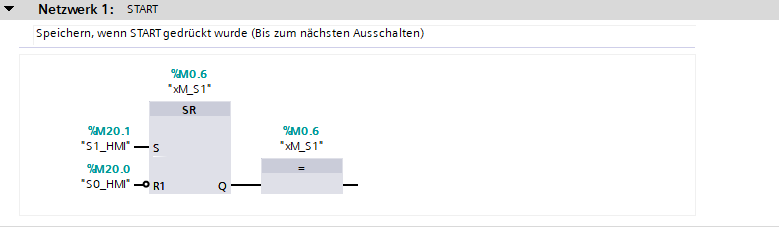
\includegraphics[width=0.8\textwidth]{Bilder/1. Hauptprogramm/main_1.png}}
   \caption[Starten der Anlage]{Starten der Anlage}
   \label{fig:Bild1.1}
\end{figure}

Im zweiten Netzwerk (\autoref{fig:Bild1.2}) wird der 5-Sekunden-Nachlauf des Förderbandes nach der Förderschnecke beim Ausschalten programmiert. Durch die Abfrage des Zustands des STOP-Leuchtdrucktasters (S0) wird das Schütz der Förderschnecke (K3) ausgeschaltet. Der STOP-Taster wurde als Öffner vorgesehen, folglich wird auf die negative Flanke getriggert. Sobald das Schütz (K3) ausgeschaltet ist, wird die Ausschaltverzögerung (TOF) gestartet. Nach Ablauf der 5-Sekunden wird das Schütz des Förderbandes (K4) ebenfalls ausgeschaltet.

\begin{figure}[H]
   \centering
   \fbox{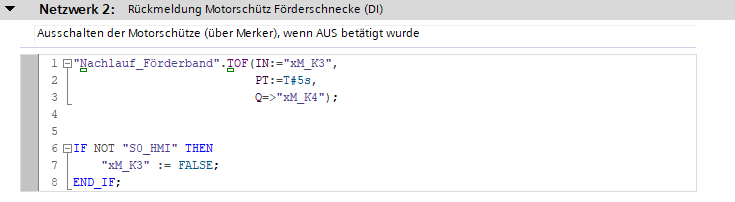
\includegraphics[width=0.8\textwidth]{Bilder/1. Hauptprogramm/main_2.png}}
   \caption[Stoppen der Anlage]{Stoppen der Anlage}
   \label{fig:Bild1.2}
\end{figure}

Im dritten Netzwerk (\autoref{fig:Bild1.3}) wurden Abfragen zu den Bedingungen für die Zustände der Anlage implementiert. Jede \textit{IF} \bzw \textit{ELSIF}-Bedingung fragt die Eintrittsvoraussetzungen eines Zustands ab. Diese können aus den Zustandsgraphen abgelesen werden. Sind die Bedingungen für einen Zustand erfüllt, wird der Funktionsbaustein \texttt{Zustände_DB()} mit einer Nummer aufgerufen. Die Nummer gibt an, um welchen Zustand es sich handelt. Folgende Zustände wurden Umgesetzt:

\begin{itemize}
    \item 0 - Betriebsbereiter Zustand
    \item 1 - Anlauf Förderband
    \item 2 - Anlauf Schnecke
    \item 3 - Schnecke Stop
    \item 4 - Förderband Stop
\end{itemize}

Der Nachlauf des Förderbandes wurde in keinem separaten Zustand umgesetzt, sondern ist in Netzwerk 2 (\autoref{fig:Bild1.2}) beim Stoppen der Anlage mit implementiert. \\
Der Anlauf der Schnecke erfolgt ebenfalls zeitverzögert (TON) und ist von Zeile 1 bis 3 im Netzwerk 3 (\autoref{fig:Bild1.3}) umgesetzt. Der Eingang der Einschaltverzögerung beinhaltet die gleichen Bedingungen wie der Zustand \textit{\glqq Anlauf Förderband\grqq{}}.

\begin{figure}[H]
   \centering
   \fbox{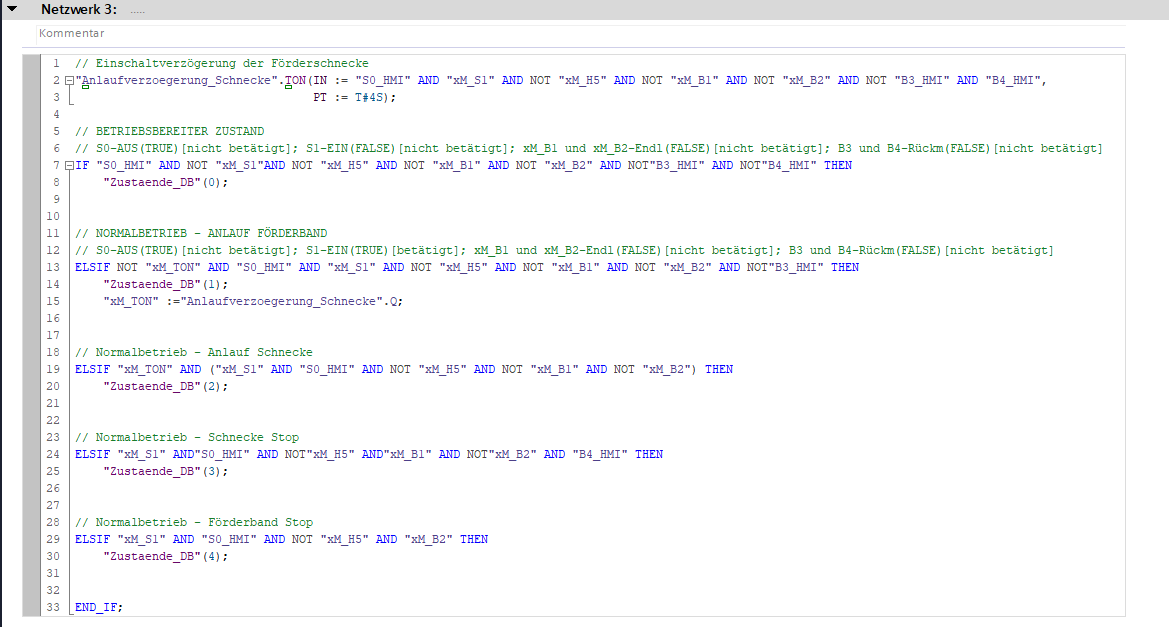
\includegraphics[width=0.95\textwidth]{Bilder/1. Hauptprogramm/main_3.png}}
   \caption[Abfrage der Zustandsbedingungen]{Abfrage der Zustandsbedingungen}
   \label{fig:Bild1.3}
\end{figure}

Das vierte Netzwerk (\autoref{fig:Bild1.4}) umfasst das Verhalten der Anlage im Fehlerfall. Dabei wird in drei Phasen unterschieden:
\begin{itemize}
    \item Fehler wird detektiert
    \item Fehler wird behoben
    \item Fehler wird quittiert
\end{itemize}

Im der ersten Phase blinkt der Leuchtmelder (H5) mit einer Frequenz von f = 1Hz. Dazu wird der Funktionsbaustein \texttt{Blinktakt()} aufgerufen. Sobald der Fehler behoben wurde, wird dies durch das dauerhafte Leuchten von H5 signalisiert. Gleichzeitig erfolgt das Blinken des QUITTIER-Leuchtdrucktasters (H2) mit selbiger Frequenz des Leuchtmelders H5 aus Phase 1. Sobald der QUITTIER-Leuchtdrucktaster (S2) gedrückt wurde, ist die Phase zwei beendet und die Anlage wird in Phase drei wieder in den betriebsbereiten Zustand versetzt.

\begin{figure}[H]
   \centering
   \fbox{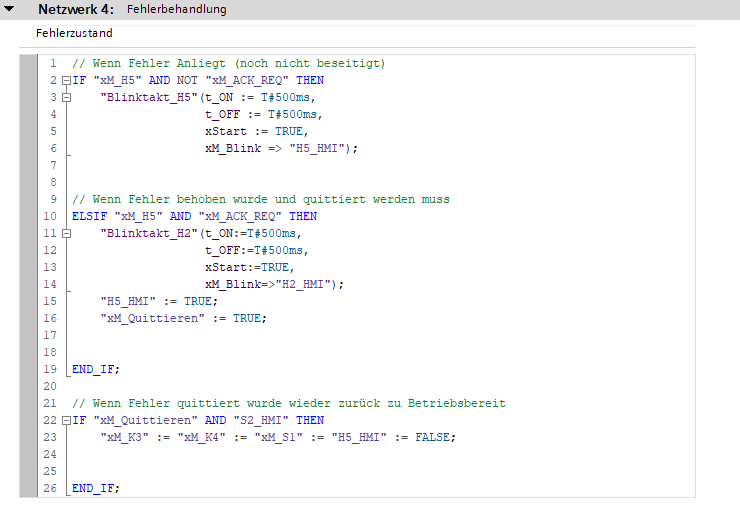
\includegraphics[width=0.8\textwidth]{Bilder/1. Hauptprogramm/main_4.png}}
   \caption[Beschreibung des Fehlerzustands]{Beschreibung des Fehlerzustands}
   \label{fig:Bild1.4}
\end{figure}

Das Netzwerk Fünf (\autoref{fig:Bild1.5}) ist lediglich im simulierten Anlagenzustand anzuwenden und ermöglicht die Rückmeldung der geschalteten Schütze (K3 und K4) durch die Variablen (B3 und B4). Im realen Anlagenbetrieb werden die Rückmeldungen automatisch durchgeführt, folglich ist dieses Netzwerk zu entfernen.

\begin{figure}[H]
   \centering
   \fbox{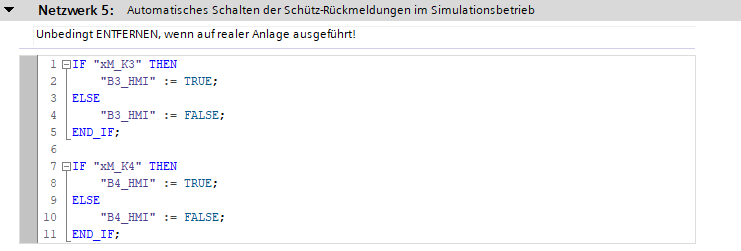
\includegraphics[width=0.8\textwidth]{Bilder/1. Hauptprogramm/main_5.png}}
   \caption[Setzen der Rückmeldungen der Schütze]{Setzen der Rückmeldungen der Schütze}
   \label{fig:Bild1.5}
\end{figure}

\subsection{Funktionsbaustein der Zustände}

Der Funktionsbaustein \texttt{Zustände_DB()} (\autoref{fig:Bild1.6}) umfasst die Implementierung der Zustände gemäß der Zustandsgraphen. Im Main-File werden entsprechend Integer-Werte von Null bis Vier vergeben. Anhand dieser Werte wird durch eine CASE-Anweisung der richtige Zustand ermittelt und die jeweiligen notwendigen Variablen auf TRUE oder FALSE gesetzt. Sofern die Anlage keinen dieser Zustände zugeordnet werden kann, wird über die ELSE-Abfrage eine Textnachricht im Terminal der SPS zurückgegeben. Die Anlage wird durch die Safety-Baugruppen ausgeschaltet und in einen sicheren Zustand versetzt.

\begin{figure}[H]
   \centering
   \fbox{\includegraphics[width=0.7\textwidth]{Bilder/1. Hauptprogramm/Zustände.png}}
   \caption[Funktionsbaustein Zustände\_DB()]{Funktionsbaustein Zustände\_DB()}
   \label{fig:Bild1.6}
\end{figure}

\subsection{Blinker-Funktionsbaustein}

Zuletzt wurde ein Funktionsbaustein für eine Blinker-Funktionalität umgesetzt (\autoref{fig:Bild1.7}). Über diesen ist es möglich per Aufruf von \texttt{Blinktakt()} ein Blinksignal zu generieren. Dem Funktionsbaustein kann eine Ein-Zeit (t\_ON) und eine Aus-Zeit (t\_OFF) mitgegeben werden, um den Blinktakt zu setzen. Über \textit{xStart} wird der Blinker aktiviert. Die Ausgangsvariable (xM\_Blink) liefert das generierte Blinksignal. \\
Eingesetzt wird der Funktionsbaustein für den \textbf{START-Leuchtdrucktaster}, den \textbf{Fehlerleuchtmelder} und den \textbf{QUITTIER-Leuchtdrucktaster}.

\begin{figure}[H]
   \centering
   \fbox{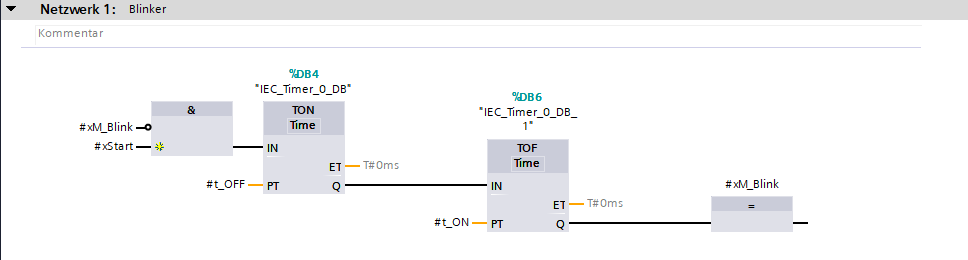
\includegraphics[width=0.8\textwidth]{Bilder/1. Hauptprogramm/Blinker.png}}
   \caption[Funktionsbaustein Blinker()]{Funktionsbaustein Blinker()}
   \label{fig:Bild1.7}
\end{figure}